% !TeX root = Project.tex
\clearpage
\noappendicestocpagenum
\begin{appendices}
% !TeX root = Project.tex

\section{List of Definitions}
Here I list some definitions which I did not have time to work into the main body of the text. The notation here mostly follows the style documented at the \href{https://en.wikipedia.org/wiki/List_of_mathematical_symbols}{Wikipedia} page for mathematical notation. Sets are normally denoted with capitals, $A, B, C\ldots$, and sets of [sub]sets in calligraphic font $\A, \B, \mathcal{C}\ldots$ Notably, the power set $\mathcal{P}(X)$ of a set X follows this pattern.

% 1
\begin{definition}[The Extended Real Line, $\eR$]\label{def:eRealLine}
$${\color{Magenta}\eR} \defeq \R \cup \{-\infty,\> +\infty\}$$
\end{definition}

% 2
\begin{definition}[$\sigma$-Algebra]\label{def:salgebra}
Given
\begin{itemize}
\item
	A set, $X$,
\item
	A family of subsets of $X$, $\A \subset \P(X)$.
\end{itemize}
Then $\A$ is a {\color{Magenta}\emph{$\sigma$-Algebra}} of $X$ $\logeq$
\begin{enumerate}[(i)]
\centering
\item
	$\emptyset \in \A$ \vspace{2pt},
\item
	$(A_j)_{j\in\N} \subset \A \Rightarrow \bigcup\limits_\N A_j \in \A$,
\item
	$A \in \A \Rightarrow  X\backslash{}A [\ \equiv A^c] \in \A$.
\end{enumerate}
\end{definition}

% 3
\begin{definition}[Measurable Space]\label{def:mablespace}
Given
\begin{itemize}
\item
	A set, $X$,
\item
	A \dref{def:salgebra}[\emph{$\sigma$-Algebra}] of $X$, $\A$.
\end{itemize}
Then
\begin{itemize}
\item
	$\text{\it The ordered pair }(X, \A) \text{\it \ is a {\color{Magenta}Measurable Space}}$.
\item
	$\text{ A set }\A \in \A \text{\it\ is {\color{Magenta}Measurable}}.$
\end{itemize}
\end{definition}

% 4
\begin{definition}[The $\sigma$-Algebra Generated by $\G, \sigma(\G)$]
Given 
\begin{itemize}
\item
	A set, $X$,
\item
	$\G \subset \P(X)$.
\end{itemize}
Then {\color{Magenta}$\sigma(\G)$} is the {\color{Magenta}\emph{$\sigma$-Algebra Generated by $\G$}} $\logeq$
\begin{enumerate}[(i)]
\centering
\item
	$\G \subset {\color{Magenta}\sigma(\G)}$,
\item
	${\color{Magenta}\sigma(\G)} \text{\it\ is a } \dref{def:salgebra}[\sigma\text{\it -Algebra}] \text{\it\ of }X$,
\item
	$\A \text{\it\ is a }\dref{def:salgebra}[\sigma\text{\it -Algebra}] \text{\it\ of } X \text{\it\ and } \G \subset \A  \Rightarrow {\color{Magenta}\sigma(\G)} \subset \A.$
\end{enumerate}
\end{definition}

% 5
\begin{definition}[The family of half open rectangles in $\R^n$, $\J$]\label{def:rect}
$$\P(\R^n) \supset {\color{Magenta}\J} \defeq \{(a_1, b_1] \times (a_2, b_2] \times \dots \times (a_n, b_n]; \; \forall a_k, b_k \in \R\}$$
\end{definition}

% 6
\begin{definition}[The Borel $\sigma$-Algebra on $\R^n, \B(\R^n)$]\label{def:balgebra}
Fix $n \in \N$. Given the family of half open rectangles $\mathcal{J}^{o,n}$
$$ \text{\it The } \dref{def:salgebra}[\sigma\text{\it -Algebra}] \text{\it\ generated by } {\color{Magenta}\mathcal{J}^{o,n}}\text{\it\ is the } \text{\color{Magenta}\it Borel $\sigma$-Algebra} \text{\it\ on }\R^n$$
\end{definition}

% 7
\begin{definition}[The Extended Borel $\sigma$-Algebra on $\eR^n, \eB(\eR^n)$]
Fix $n \in \N$. $S^* \in {\color{Magenta}\eB} \logeq$
$$\exists B \in \B(\R) \text{\it\ and }\exists S \in \{\emptyset,\> +\infty,\> -\infty, \{+\infty, -\infty\}\}: \quad S^* = B \cup S$$
\end{definition}

% 8
\begin{definition}[Measures]\label{def:measure}
Given 
\begin{itemize}
\item
	A \dref{def:mablespace}[\emph{Measurable Space}], $(X, \A)$,
\item
	A map, $\mu\colon \A \rightarrow \R$.
\end{itemize}
$\text{Then } {\color{Magenta}\mu} \text{ is a} {\color{Magenta}\emph{ Measure }} \text{on the \dref{def:mablespace}[\emph{Measurable Space}] } (X, \A) \logeq$
\begin{enumerate}[(i)]
\centering
\item
	${\color{Magenta}\mu}(\emptyset) = 0$
\item
	$A, B \in \A; \> A \cap B  = \emptyset \quad \Rightarrow \quad {\color{Magenta}\mu}(A \cup B) = {\color{Magenta}\mu}(A) + {\color{Magenta}\mu}(B)$
\end{enumerate}
\end{definition}

% 9
\begin{definition}[Measure Space]\label{def:mspace}
Given
\begin{itemize}
\item
	A \dref{def:mablespace}[\emph{Measurable Space}], $X$,
\item
	A \dref{def:measure}[\emph{Measure}], $\mu$, on $(X, \A)$.
\end{itemize}
Then
$$\text{\it The ordered triple }(X, \A, \mu) \text{\it \ is a } {\color{Magenta}\emph{Measure Space}}.$$
\end{definition}


% 10
\begin{definition}[{[Discrete]} Probability Space]\label{def:pspace}
Given
\begin{itemize}
\item[\tiny$\otimes$]
	$(\omega_n)_{n \in \N} = \Omega$ [\emph{for a Discrete Probability Space}],
\item
 	A \dref{def:mspace}[\emph{Measure Space}], $(\Omega, \A, p)$.
\end{itemize}
Then $(\Omega, \A, p)$ is a {\color{Magenta}\emph{[Discrete] Probability Space}} and {\color{Magenta}$p$} a {\color{Magenta}\emph{Probability Measure}} $\logeq$
\begin{itemize}
\centering
\item[]
	$p(\Omega) = 1$.
\item[]
	(ii*) \ \ $\bigcup\limits_\N \mu(\{\omega_n\}) = 1$ \emph{[Discrete]}.
\end{itemize}
\end{definition}

% 11
\begin{definition}[The Lebesgue Measure $\lambda^n$]\label{def:lmeasure}
Fix $n \in \N.$ Given 
\begin{itemize}
\item
	The \dref{def:mablespace}[\emph{Measurable Space}], $\bigl(\R^n, \B(\R^n)\bigr)$,
\item
	A \dref{def:measure}[\emph{Measure}], $\lambda^n$, on $\bigl(\R^n, \B(\R^n)\bigr)$.
\end{itemize}
Then {\color{Magenta}$\lambda^n$} is the {\color{Magenta}\emph{Lebesgue Measure}} on $\bigl(\R^n, \B(\R^n)\bigr) \logeq$ 
$$\forall X \in \J\!, \quad {\color{Magenta}\lambda^n(X)} = \prod_{k=0}^n(b_k - a_k).$$
\end{definition}

% 12
\begin{definition}[Measurable Mapping]\label{def:mmap}
Given
\begin{itemize}
\item
	\dref{def:mablespace}[\emph{Measurable Spaces}], $(X, \A)$ and $(X', \A')$,
\item
	A map, $T\colon X \rightarrow X'$.
\end{itemize}
Then {\color{Magenta}$T$} is an {\color{Magenta}\emph{$(\A/\A')$-Measurable Map}} $\logeq$
$$ A' \in \A' \Rightarrow T^{-1}(A') \in \A.$$
\end{definition}

% 13
\begin{definition}[Image Measure]\label{def:imeasure}
Given
\begin{itemize}
\item
	\dref{def:mablespace}[\emph{Measurable Spaces}], $(X, A), \> (X', \A')$,
\item
	A \dref{def:mmap}[\emph{Measurable Mapping}], $T\colon X \rightarrow X'$,
\item
	An \dref{def:measure}[\emph{Measure}], $\mu$, on $(X, A)$.
\end{itemize}
Then,
$${\color{magenta}\mu'\colon} \A' \rightarrow \R, \>\> A \mapsto \mu\bigl({T}^{-1}(A')\bigr) \text{\it\ is the {\color{Magenta}Image Measure} of $\mu$ under {$T$}}.$$
\end{definition}

% 14
\begin{definition}[Measurable {[Numerical]} Function]\label{def:mfun}
Fix $n \in \N$. Given
\begin{itemize}
\item
	\dref{def:mspace}[\emph{Measure Space}], $(X, \A), \> (X', \A')$,
\item
	An \dref{def:mmap}[\emph{$(\A/\A')$-Measurable Mapping}], ${\color{Magenta}u}\colon X \rightarrow X'$.
\end{itemize}
Then, if $(X', \A') = \bigl(\R, \B(\R)\bigr) \>\, [\,\bigl(\eR, \eB(\eR)\bigr)\,]$,
$${\color{Magenta}u} \text{\it\ is an {\color{Magenta}$(\A/\B [\eB])$-Measurable [Numerical] Function}, } {\color{Magenta}u}\colon X \rightarrow \R \> [\eR]$$
\end{definition}

% 15
\begin{definition}[{[Real-Valued]} Random Variable]\label{def:rvariable}
Given 
\begin{itemize}
\item
A \dref{def:pspace}[\emph{Probability Space}], $(\Omega, \A, p)$, and a \dref{def:mablespace}[\emph{Measurable Space}], $(X[=\R], \A')$,
\item
An \dref{def:mmap}[\emph{$(\A/\A')$-Measurable Mapping}], ${\color{Magenta}Y}\colon\Omega \rightarrow X[= \R]$.
\end{itemize}
Then {\color{Magenta}$Y$} is a {\color{Magenta} \emph{[Real-Valued] Random Variable}}.  The \dref{def:imeasure}[\emph{Image Measure}] of $p$ under $Y$ gives the {\color{Magenta}\emph{Probabilities}} of the {\color{Magenta}\emph{Events,} $E$} $\in \A'.$ 
\end{definition}

% 16
\begin{definition}[Simple Function]\label{def:sfun}
Given
\begin{itemize}
\item
	A \dref{def:mablespace}[\emph{Measurable Space}], $(X, \A)$ along with $\measurespace$,
\item
	An \dref{def:mfun}[\emph{$(\A, \B)$-Measurable Function}], $u: X \rightarrow \R.$
\end{itemize}
Then $u$ is a {\color{Magenta}\emph{Simple Function}} $\logeq$
$$\exists N \in \N: \> \exists(A_j)_{j=0}^N \text{\it\ with } A_j \in \A \text{\it\ and } \> \exists(c_j)_{j=0}^N \text{\it\ with } %
c_j \in \R \> : u(x) = \sum_{j=0}^N c_j \cdot \indi[A_j] \;\; \forall x \in X$$.
Given a measure, $\mu$, on the space $(X, \A)$; {\color{Magenta}\emph{the set of all Simple Functions}} on $(X, \A, \mu)$ is {\color{Magenta}\emph{$\E_\mu$}}. {\color{Magenta}\emph{the set of all non-negative Simple Functions}} is {\color{Magenta}\emph{$\E_\mu^+$}}.
\end{definition}

% 17
\begin{definition}[Integral of a Simple Function]\label{def:sint}
Given
\begin{itemize}
\item
	A \dref{def:mspace}[\emph{Measure Space}], $(X, \A, \mu)$,
\item
	A non-negative \dref{def:sfun}[\emph{Simple Function}], $s\colon X \rightarrow \R_{\geq 0}$,
\item
	$N \in \N$,
\item
	Sets, $(A_j)_{j=0}^N$ and $(c_j)_{j=0}^N : s(x) = \sum_{j=0}^N c_j \cdot \indi[A_j] \;\; \forall x \in X$.
\end{itemize}
Then {\color{Magenta}$I_\mu$(s)} is the {\color{Magenta}\emph{Integral of the Simple Function}}, $s$, where
$${\color{Magenta}I_\mu(s)} = \sum_{j=0}^N c_j \cdot \mu(A_j)$$
\end{definition}
% !TeX root = Project.tex
\section{Approximating area --- Riemann Style}

This is the code I wrote to draw the sequence of approximations shown in Figure \ref{fig:areaapprox}. It can be used to visualise the approximation of the Integral of any function in a \dref{def:riemann}[\emph{`Riemann style'}] --- given that you already have a way to write it as a Python function with the form:

\begin{minted}{python}
# f(x) -----> number.
\end{minted}

It can be modified easily to produce quite a few of approximations - here we just set n to 6.

\begin{minted}{python}
import matplotlib.pyplot as plt
import numpy as np 

n = 6
\end{minted}

First, we want to set the limits of integration, $[a, b]$, and use this to calculate a total width.

\begin{minted}{python}
xmax = 6
xmin = 0
totalwidth = xmax - xmin
\end{minted}

Then we use this, and our n, to split up the axis into $5 \times 2^{n-1}$ equal sized sections. We will divide the lengths of each bar by 2 every step of the approximation, so this ensures that our coarsest approximation has 5 bars. 
\begin{minted}{python}
# 160 points equally spaced points (plus zero) in the domain
num = (5 * 2**(n-1)) + 1
x = np.linspace(xmin, xmax, num=num, endpoint=True)
\end{minted}

Define the function of interest, $f$.
Calculate $y$ values to plot a graph. 

\begin{minted}{python}
# Make a list of 'n' colours
colour1 = '#95d0fc' #light blue
colour2 = '#75bbfd' #sky blue
colour3 = '#00ffff' #cyan
colour4 = '#13eac9' #aqua
colour5 = '#929591' #grey
colour6 = '#06c2ac' #turquoise
colour = [colour1, colour2, colour3, colour4, colour6, colour5]

f = np.sin
y = f(x)

# To draw graph
xs = np.linspace(xmin, xmax, 100)
ys = f(xs)

fig, axesr = plt.subplots(nrows=int(n/2), ncols=2, dpi=300, figsize=(5, n*3/4))
fig.subplots_adjust(hspace = 0.075)
axes = [ax for axes in axesr for ax in axes]

fig.subplots_adjust(wspace=0.05, hspace=0.075)

for ax in axes:
    ax.plot(xs, ys, 'g-', linewidth=0.5) 
    ax.tick_params(top=False, 
                   bottom=False, 
                   left=False, 
                   right=False, 
                   labelleft=False, 
                   labelbottom=False, 
                   labelright=False,
                   labeltop=False)
    for axis in ['top','bottom','left','right']:
      ax.spines[axis].set_linewidth(0.4)

    ax.set_xlim(xmin, xmax)    
\end{minted}
    
A quick explanation of this next step is that it's setting up the \dref{def:stfun}[\emph{`representations'}] of the
\dref{def:stfun}[\emph{Step Functions}] used to approximate the function of interest. Those sequences are defined by $$x_{n,m} = x_{n,m-1} + \frac{totalwidth}{5 \times 2^{n-1}}$$

In this example, I am bounding the function from below, but by changing 'min' to 'max', you can bound it from above.

\begin{minted}{python}
reps = [x[:-1:2**n] for n in range(n)]
bars = [(x, []) for x in reps]
for interval_steps, bar in zip(reps, bars):
    for i in range(len(interval_steps)):
        xright = xmax if i == len(interval_steps) - 1 else interval_steps[i+1]
        xleft = interval_steps[i]
        interval = np.linspace(xleft, xright, 1000)
        interval_mapped = [f(x) for x in interval]
        interval_min = min(interval_mapped) ## Can change 'min' to 'max'
        bar[1].append(interval_min)         ## to bound from above
\end{minted}
      
Now we can plot the bars at the right heights, using the colours we picked earlier.  Also, what I mean by \emph{`bounding from below'} is that we are finding the \dref{def:hseq}[\emph{height sequence}] where every height is the greatest lower bound (infinium) of the values the function takes in the corresponding step. But that's a bit of a mouthful.

\begin{minted}{python}
i = n
for ax in reversed(axes):
    i -= 1
    div = 5 * 2**i
    ax.bar(*bars[n-i-1], 
        align='edge', width=(totalwidth/div), 
        fc=colour[i], ec=colour[i], alpha=0.95)

fig.savefig('RiemannExample.png')
\end{minted}

\begin{figure}[H]
\centering
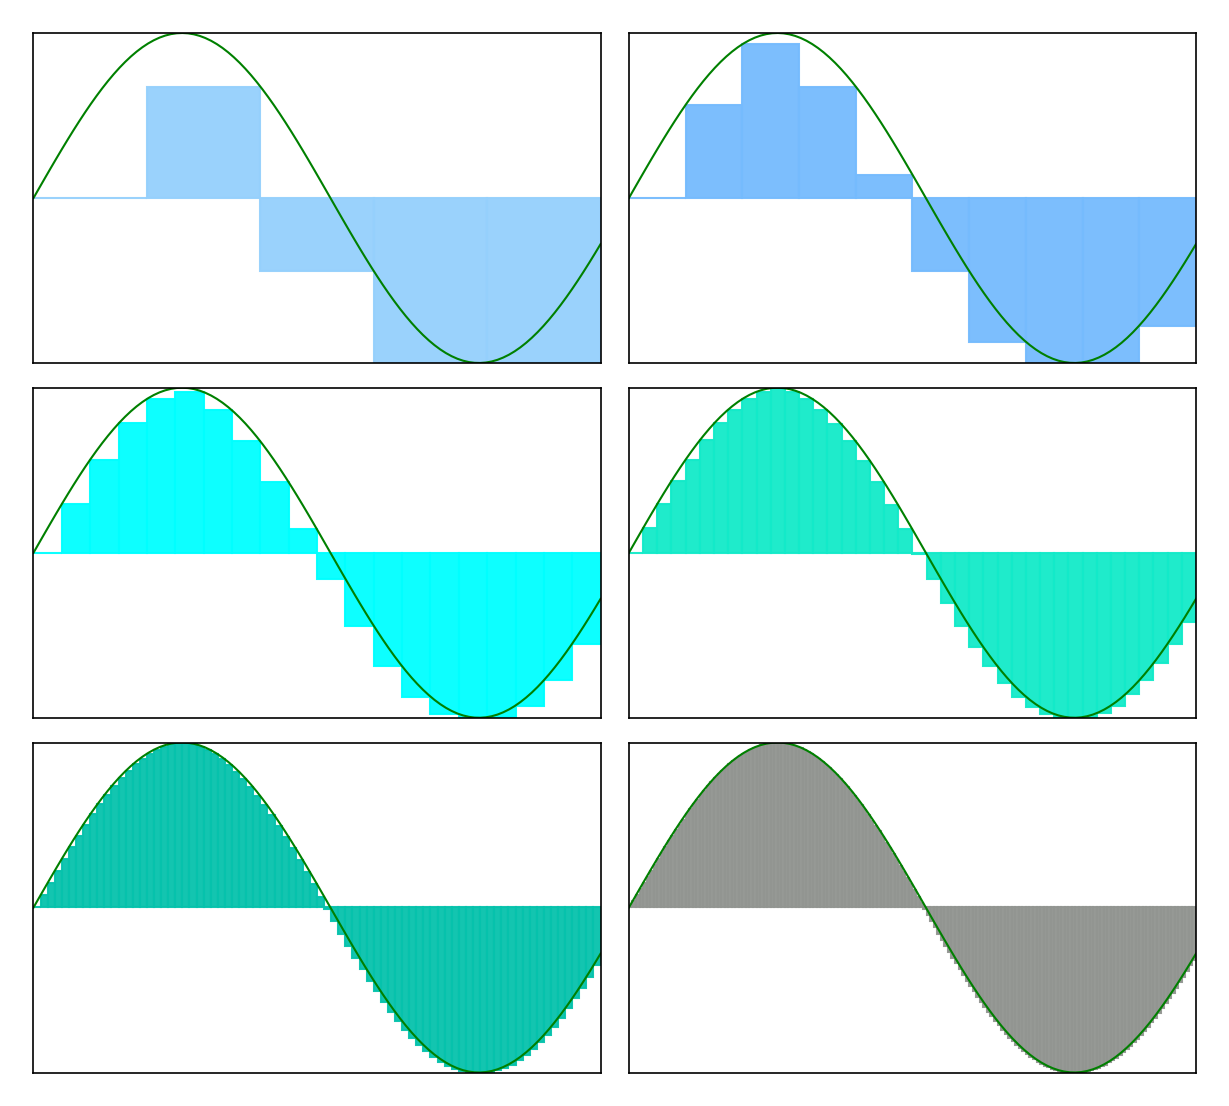
\includegraphics{Code/RiemannExample.png}
\caption{RiemannExample.png}
\end{figure}
% !TeX root = Project.tex
\newpage
\section{Approximating Area --- Lebesgue Style}

This is the code I used to draw the sequence of approximations shown on the Title Page and in the Abstract. It can be used to visualise approximating the integral of any \dref{def:mfun}[\emph{positive Measurable Function}] in a \dref{def:main}[\emph{`Lebesgue Style'}], given that you have a way to write it as a simple Python function with the form:"

\begin{minted}{python}
# f(x) -----> non-negative number.
\end{minted}

It can be modified easily to produce quite a few approximations. Here we do 5.

\begin{minted}{python}
import matplotlib.pyplot as plt
import matplotlib.patches as patches
import numpy as np
import matplotlib.cm as cm
from scipy.interpolate import interp1d
from mpl_toolkits.axes_grid1.axes_divider import make_axes_locatable

# How many approximations?
STEPS = 5
\end{minted}

In a sense, we are actually doing 2 stages of approximation. The first is that, instead of working with $(\R^n, \B(\R^n))$ and finding the actual \dref{def:main}[\emph{Lebesgue Integral}], I discretise the domain --- i.e. split it into equal sized sections, and focus on some point in the middle --- and give each point a measure that is proportional the size of each section.

\medskip
If you're smarter than me, and have more time than I do, you could do everything I do below for a rectangle in $R^n$ by dividing the domain into squares, or cubes, etc., and numbering each one. In this case, I split the domain into 500 sections. If the total length of the domain is $l$, each point $x_n$ has a measure of $\frac{l}{500}$. 

\begin{minted}{python}
GRAN = 500
X_MIN = 0
X_MAX = 10
POINT_SIZE = (X_MAX-X_MIN)/GRAN
\end{minted}

The second stage of approximation is where things get interesting. Here is where we approximate the given function as a sequence of \dref{def:sfun}[\emph{Simple Functions.}]. Technically, because of the first approximation, our new function is already a Simple Function --- any finite number of points in the domain means that we could always just define the function as $$\sum_{\text{all } x}\mathbbm{1}_{\{x\}}\cdot g(x) $$ 
But the point is that this method could be used on \emph{any} \dref{def:mfun}[\emph{Measurable Function}]; however I personally don't have a way to write a python function that says 'Find the all the elements in the potentially uncountable set of inverses of $y$, $f^{-1}(y)$, and then measure that set. The idea behind this method of approximation is as follows:

\medskip
Lets imagine we have a totally random \dref{def:mspace}[\emph{Measure Space}], $(X, A, \mu)$, and a \dref{def:mfun}[\emph{non-negative Measurable Function}], u, on that space.

\medskip
The goal is to approximate the area in increasing steps, with every step getting closer to the true value.

\medskip
At each step in the approximation, $n$ (starting at 0), we will focus on the function below a certain (strictly-increasing) height. Specifically, $n$ itself.

\medskip
Above this height, we will just give the Simple Function the value zero - but the higher we go, the better the approximation. Moreover, if $f$ is bounded, then we are guaranteed to eventually reach a height where all the points are accounted for.

\medskip
At every step we divide the range below $n$ into $n \cdot 2^{n}$ equal sized levels, so that between 0 and 1, for instance, there are $2^{n}$ levels. Notice that with each step, the level sets are getting finer.

\medskip
Fix an $n$. Now, let $$y_{n,j} = y_j = j \cdot 2^{-n} \quad \forall j \in \N_{\leq n2^n} \cup \{0\}, $$ so that the $y_{n,j}$s are the points where split the domain into levels.

\medskip
For all $y_j$ except the last one, find 'level sets' $$X_j = \{x : f(x) \in [y_j, y_{j+1})\}$$ . i.e. find $$f^{-1}([y_j, y_{j+1}))$$

\medskip
The Simple Function, $s_n$, which we use to approximate the area is then $$\sum_{j=0}^{j=n\cdot2^{n - 1}} y_j \cdot \mathbbm{1}_{X_j}(x)$$ Note that since $f$ is a Measurable Function, and since all $(a, b)$ in the space $(\R, \B)$ are Measurable, we must have $$f^{-1}((y_j, y_{j+1})) \in \A.$$ That's why this works, and why $f$ (or $u$ or whatever I'm calling it) needs to be a \dref{def:mfun}[\emph{positive Measurable Function}].

\medskip
We then find $\dref{def:sint}[I_{\mu}(s_n)]$ using the \dref{def:measure}[\emph{Measure}] $\mu$ on $X$.

\medskip
In our case, instead of using the \dref{def:lmeasure}[$\lambda$\emph{-Measure}] on $\R$, we have to use a simplified and discretised Measure Space - but one that gets 'closer' to $\lambda$ the more points you pick.

\medskip
With all that out of the way, lets do my favorite part in all this, and pick the colours.

\begin{minted}{python}
def colour(x=1.0):
    r = list(cm.rainbow(x/STEPS))
    r[3] = 0.5  # I think it looks better with a lower 'alpha'
    return tuple(r)

# We will be calculating 2^(-n) a lot to figure out the step size
# So this is a function to do that
def ss(x):
    return 2**(-x)

# Set up the graph and function.
# Our graph in this case is drawn by interpolation,
# but you can change the definition of f to any function
# which takes a float and returns another float.
xi = np.linspace(X_MIN, X_MAX, num=5, endpoint=True)
yi = [0, 1.75, 0.9, 2.5, 2.5]
f = interp1d(xi, yi, kind='cubic')
# The points we use to plot our graph
# and find the inverses of the levels; the level sets
def f2(x):
    return (np.sin(x) + 1.5) * 3/2
f = f2
xs = np.linspace(X_MIN, X_MAX, num=GRAN+1, endpoint=True)
ys = f2(xs)

# Set up the axes.
# For the first half
fa1 = plt.subplots(nrows=STEPS, dpi=300, figsize=(5, STEPS*3))
fig1, axes1 = fa1
# For the second half
fa2 = plt.subplots(nrows=STEPS, dpi=300, figsize=(5, STEPS*3))
fig2, axes2 = fa2

for fig in [fig1, fig2]:
    fig.subplots_adjust(wspace=0.075, hspace=0.075)

for fig, axes in [fa1, fa2]:
    for ax in axes:
        ax.set_xlim(X_MIN, X_MAX)
        ax.set_ylim(0, 4) # For this example specifically
        ax.tick_params(
           axis='both',
           which='both',
           bottom=False,
           top=False,
           left=False,
           labelleft=False,
           labelbottom=False)

###

# Calculate the level_sets.
# Code makes this easy, the difficulty is in how to organise the data
# The way I do it here is for every step in the the approximation, n,
# I have a dictionary with key vaule pairs 
#                           y_j : X_j = f^(-1)([y_j, y_j+step_size))
# And those dictionaries are kept in another dictionary called 
# all 'level_sets'. So all_level_sets[n][y_base] gives the level set
# for [y_base, y_base + step_size) for the step n
all_level_sets = {}
for j in range(1, 1+STEPS):
    step_size = ss(j)
    y_bases = np.arange(0, j, step_size)
    level_sets = {}
    for y_base in y_bases:
        X = [x for x in xs if \
             f(x) >= y_base and f(x) < y_base + step_size]
        level_sets[y_base] = X
    all_level_sets[j] = level_sets

# For the first figure, we want to visualise what's going on by colouring
# the different levels, and then underneath the graph the we show the level
# sets in matching colours. Unfortunately, since some many points overlap,
# this might not be obvious...
for step, ax in enumerate(axes1, 1):
    ax.plot(xs, ys, color='0.1', lw=0.5, linestyle='-')
    step_size = ss(step)
    y_bases = np.arange(X_MIN, step, step_size)
    for y_base in y_bases:
        ax.axhspan(y_base, y_base + step_size, # Colour the different levels 
            facecolor=colour(y_base), 
            edgecolor='none')
        if y_base >= 1 and y_base <= 1.5: # Highlight this section 
            ax.axhline(y_base, 
                       lw=0.5, 
                       color='k', 
                       alpha=0.7, 
                       linestyle='-.'
                      )
#            ax.axhspan(y_base, y_base + step_size,
#                       facecolor=colour(y_base), 
#                       edgecolor='none'
#                      )
            
    # Add a colour bar at the bottom, showing the different level
    # sets in different colours.
    # I wish I had a better way to do this...
    ax_divider = make_axes_locatable(ax)
    cax = ax_divider.append_axes("bottom", size="3%", pad="2%")
    cax.set_xlim(0,10)
    cax.set_ylim(0,0.1)
    cax.tick_params(
    axis='both',       
    which='both',      
    bottom=False,      
    top=False,         
    left=False,
    labelleft=False,
    labelbottom=False) 
    cax.axis('off')
    for y_base in np.arange(X_MIN, step, step_size):
        xmatch = all_level_sets[step][y_base]  
        cax.scatter(xmatch, [0.05]*len(xmatch), 
                    s=15, c=[colour(y_base)], marker='s')   

# For the second figure, we'd like to rearrange points in the domain, so
# that points in the same level set are next to each other.
# This can be done by just counting the number of points in a level set,
# then making a rectangle which has a width to this size.
for step, ax in enumerate(axes2, 1):
    step_size = ss(step)
    y_bases = np.arange(X_MIN, step, step_size)
    left_edge = 0
    for y_base in y_bases:
        no_of_xs = len(all_level_sets[step][y_base])
        measure = POINT_SIZE * no_of_xs
        # Draw boxes around the rectangles correspoding to the highlighted 
        # level sets.
        right_edge = measure
        rect = patches.Rectangle((left_edge, 0),
                                 measure,
                                 height=y_base,
                                 color=colour(y_base))
        if y_base >= 1 and y_base < 1.5:
            rect.set_edgecolor('k')
        ax.add_patch(rect)
        left_edge += measure
fig1.savefig('LebesgueExample1.png')
fig2.savefig('LebesgueExample2.png')
\end{minted}

\begin{figure}[H] 
	\renewcommand{\subfigcapskip}{-5pt}
	\centering
	\subfigure[LebesgueExample1.png]{%
		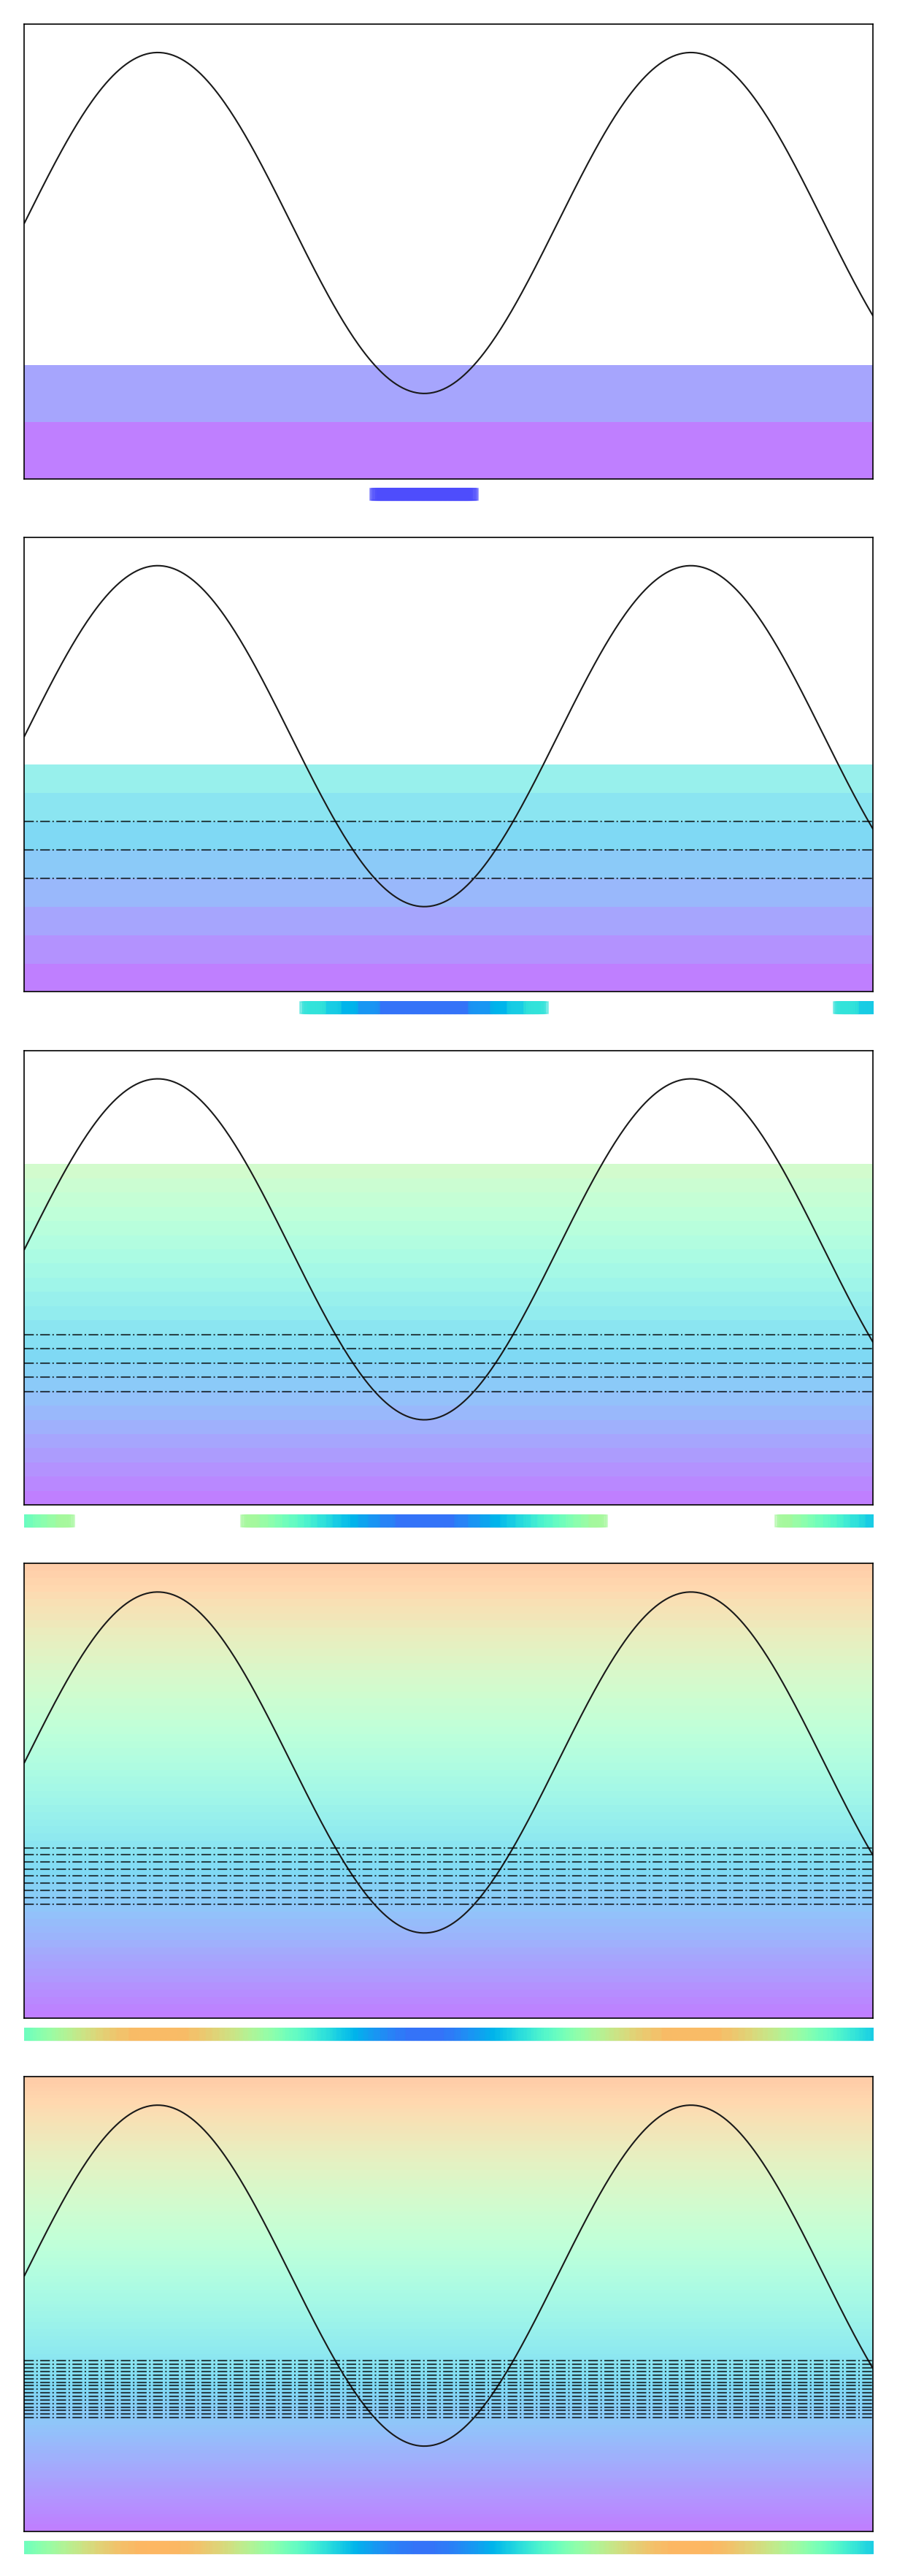
\includegraphics[scale=0.5]{Code/LebesgueExample1.png}}
	\subfigure[LebesgueExample2.png]{%
		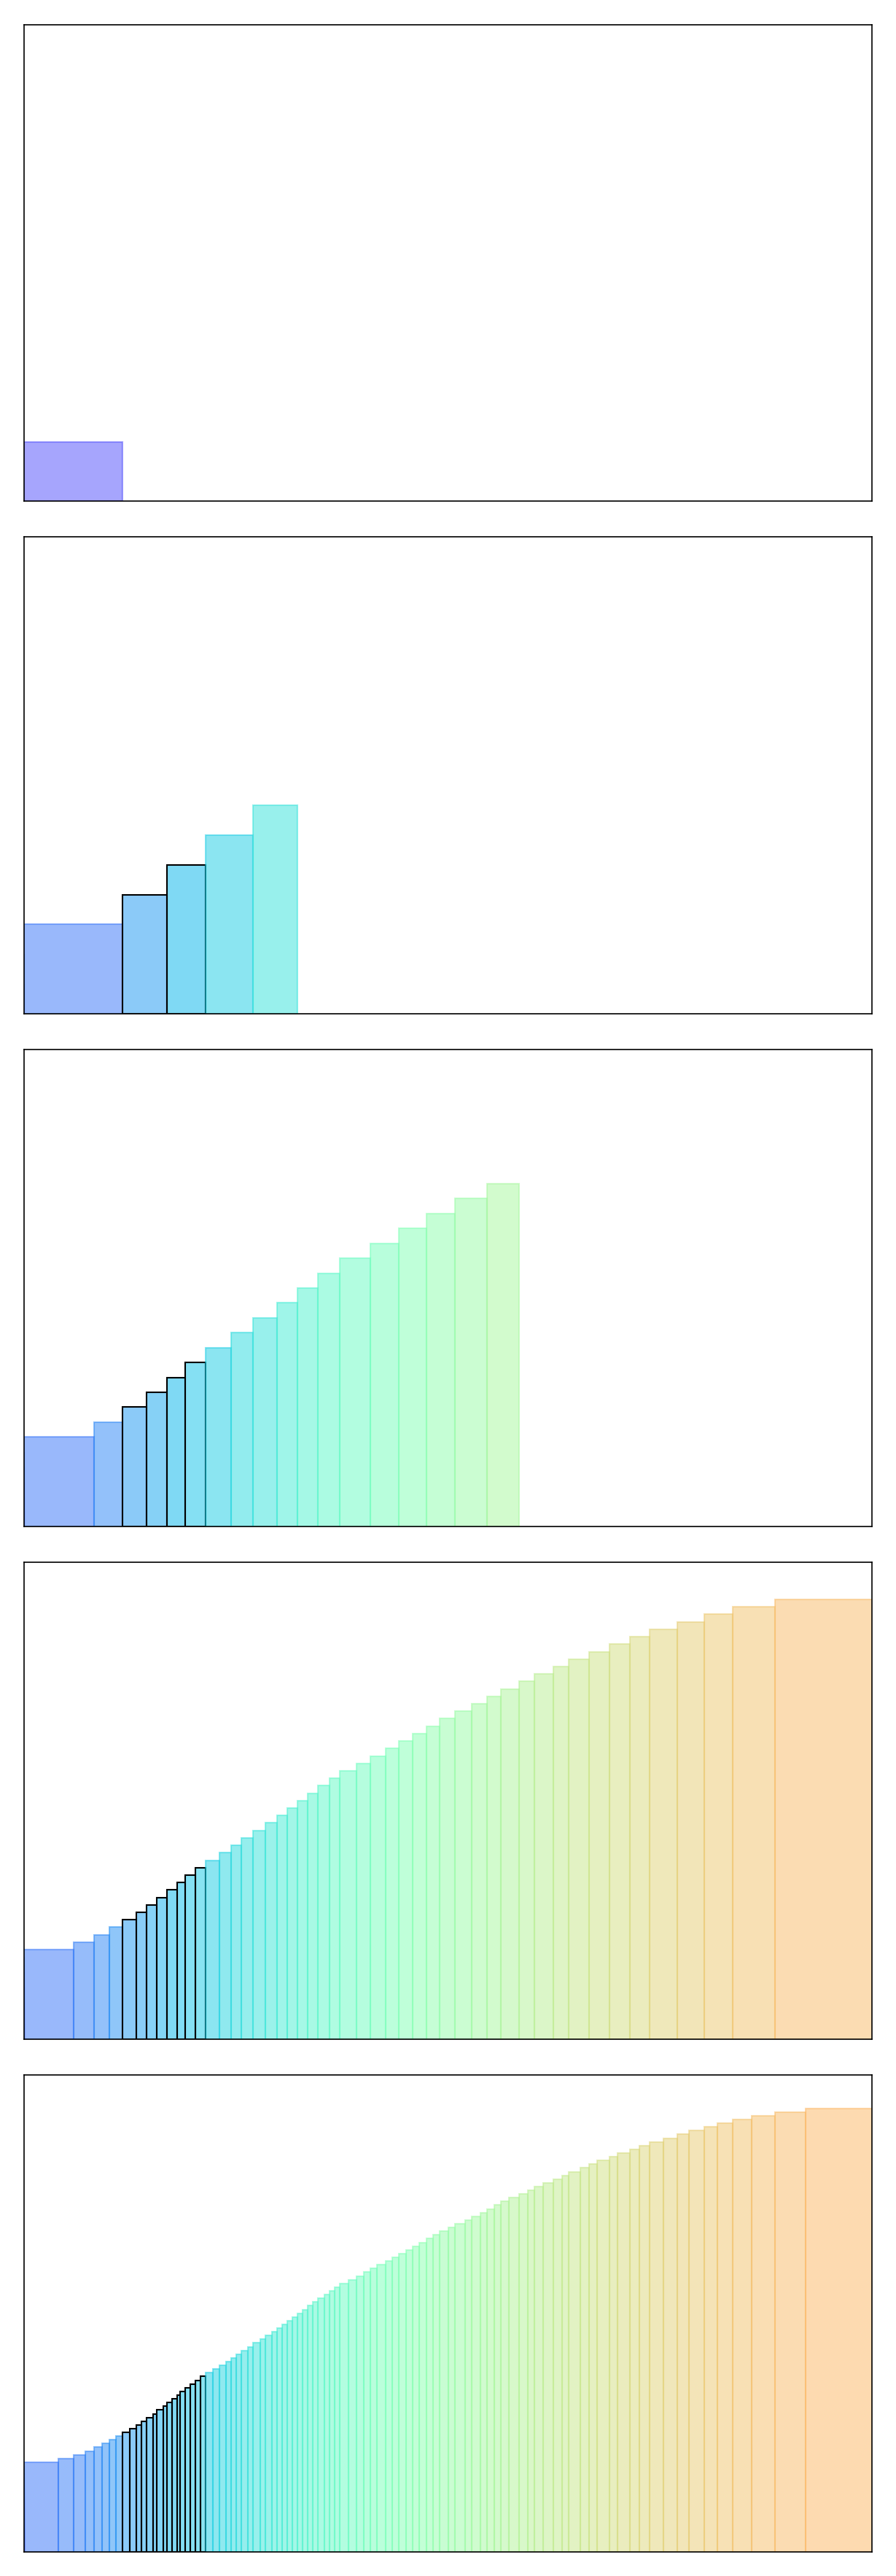
\includegraphics[scale=0.5]{Code/LebesgueExample2.png}}
	\caption{Approximating Area with Simple Functions.}
\end{figure}
\end{appendices}

\begin{bibdiv}
\begin{biblist}
\bib{MR2200059}{book}{
   author={Schilling, Ren\'{e} L.},
   title={Measures, integrals and martingales},
   publisher={Cambridge University Press, New York},
   date={2005},
   pages={xii+381},
   isbn={978-0-521-61525-9},
   isbn={0-521-61525-9},
   review={\MR{2200059}},
   doi={10.1017/CBO9780511810886},
}
\bib{MR2129625}{book}{
   author={Stein, Elias M.},
   author={Shakarchi, Rami},
   title={Real analysis},
   series={Princeton Lectures in Analysis},
   volume={3},
   note={Measure theory, integration, and Hilbert spaces},
   publisher={Princeton University Press, Princeton, NJ},
   date={2005},
   pages={xx+402},
   isbn={0-691-11386-6},
   review={\MR{2129625}},
}
\bib{youben}{webpage}{
  author={Garside B},
  title={Probability Theory},
  date={2014},
  url={https://www.youtube.com/playlist?list=PLAvgI3H-gclbyWnE9WrSq68_HRW9rOZUw},
  note={A video series on Probability}
}
\bib{settheory}{book}{
   author={Weiss, William},
   title={An Introduction To Set Theory},
   publisher={CreateSpace Independent Publishing Platform},
   date={2014},
   isbn={1502970597},
}
\bib{MR1772332}{book}{
   author={Carothers, N. L.},
   title={Real analysis},
   publisher={Cambridge University Press, Cambridge},
   date={2000},
   pages={xiv+401},
   isbn={0-521-49756-6},
   review={\MR{1772332}},
   doi={10.1017/CBO9780511814228},
}

\end{biblist}
\end{bibdiv}
